% Illustrative exact-coordinate unit triangle; no numerical-search result.
% Requires tikz and decorations.pathreplacing.
\begin{figure}[tb]
\centering
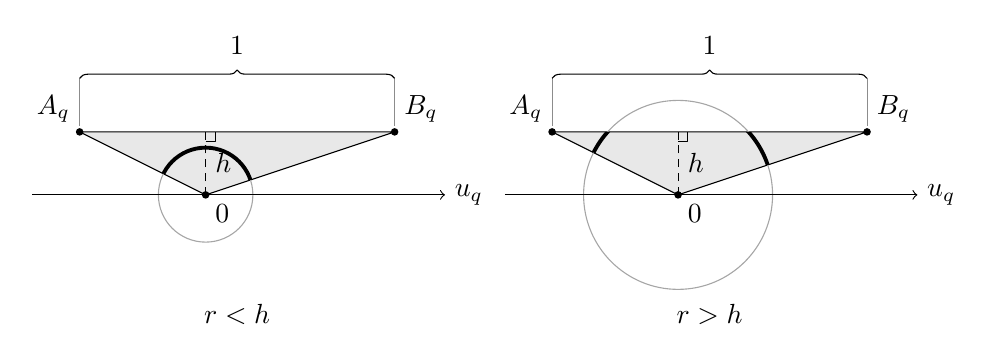
\begin{tikzpicture}[x=4cm,y=4cm,line join=round]
\foreach \rad/\shift/\tag in {0.15/0/{r<h},0.30/6/{r>h}} {
 \begin{scope}[xshift=\shift cm]
  \coordinate (O) at (0,0);
  \coordinate (Far) at (0.6,0.2);
  \coordinate (Near) at (-0.4,0.2);
  \fill[black!9] (O)--(Far)--(Near)--cycle;
  \draw[thin] (O)--(Far)--(Near)--cycle;
  \draw[black!35] (O) circle (\rad);
  \begin{scope}
   \clip (O)--(Far)--(Near)--cycle;
   \draw[line width=1.4pt] (O) circle (\rad);
  \end{scope}
  \draw[densely dashed] (O)--(0,0.2) node[midway,right] {$h$};
  \draw[thin] (0,0.17)--(0.03,0.17)--(0.03,0.2);
  \draw[->,thin] (-0.55,0)--(0.76,0) node[right] {$u_q$};
  \draw[black!45,thin] (-0.4,0.22)--(-0.4,0.37) (0.6,0.22)--(0.6,0.37);
  \draw[decorate,decoration={brace,amplitude=3pt}] (-0.4,0.37)--(0.6,0.37)
    node[midway,above=5pt] {$1$};
  \fill (O) circle (0.012) node[below right] {$0$};
  \fill (Far) circle (0.012) node[above right] {$B_q$};
  \fill (Near) circle (0.012) node[above left] {$A_q$};
  \node at (0.10,-0.38) {$\tag$};
 \end{scope}
}
\end{tikzpicture}
\caption{同一完整单位针在两个半径上的截面。浅色是原点三角形，粗圆弧是它的实际圆周截面。左图的圆周尚未达到底边，远端和近端使用同一完整角域；右图的圆周跨过底边后，截面分成两条端部弧。对两个端点计数，不意味着可以将左图的同一条粗弧计算两次。}
\label{fig:needle-sections}
\end{figure}
